% INFORMATIONEN ZUR LIZENZ
% ========================
%
% Das Dokument steht unter der Lizenz: Creative Commons by-nc-sa Version 4.0
% http://creativecommons.org/licenses/by-nc-sa/4.0/deed.de
%
% Nach dieser Lizenz darf das Dokument beliebig kopiert und bearbeitet werden,
% sofern das Folgeprodukt wiederum unter gleichen Lizenzbedingungen vertrieben
% und auf die ursprünglichen Urheber verwiesen wird.
% Eine kommerzielle Nutzung ist ausdrücklich ausgeschlossen.
%
% Die Namensnennung durch einen Verweis und die Lizenzangabe der ursprünglichen
% Urheber auf den Materialien für Schülerinnen und Schüler ist erforderlich.
%
% AUTOREN:
%  * Johannes Pieper
%  * Heiner Stroick


\documentclass[usenames,dvipsnames]{beamer}

\usepackage[utf8]{inputenc}
\usepackage[ngerman]{babel}
\usepackage[T1]{fontenc}
\usepackage{eurosym}
\usepackage{lmodern}
\usepackage{paralist}
\usepackage{schulinf}
\usepackage{listings}
\usepackage[german=guillemets]{csquotes}	
\usepackage{hyperref}
\hypersetup{
colorlinks = false,
pdftitle = Modellierung mit Objekten zum Anfassen (WS26) -- Informatik-Tag NRW 2017,
pdfsubject = OOM in Java / Groovy in der Schule mit Objekten zum Anfassen,
pdfauthor = Johannes Pieper und Heiner Stroick,
}
\usepackage{mdframed}
\usepackage{color}
\usepackage{colortbl}
\usepackage{graphicx}
\usepackage{booktabs}
\usepackage{todonotes}

\newcommand \etal{et.\,al.\xspace }
\newcommand \Seite{S.\,}

\newcommand{\RM}[1]{\MakeUppercase{\romannumeral #1{}}}

\mode<presentation> {

%\usetheme{default}
%\usetheme{AnnArbor}
%\usetheme{Antibes}
%\usetheme{Bergen}
%\usetheme{Berkeley}
%\usetheme{Berlin}
%\usetheme{Boadilla}
%\usetheme{CambridgeUS}
%\usetheme{Copenhagen}
%\usetheme{Darmstadt}
%\usetheme{Dresden}
%\usetheme{Frankfurt}
%\usetheme{Goettingen}
%\usetheme{Hannover}
%\usetheme{Ilmenau}
%\usetheme{JuanLesPins}
%\usetheme{Luebeck}
%\usetheme{Madrid}
%\usetheme{Malmoe}
%\usetheme{Marburg}
%\usetheme{Montpellier}
%\usetheme{PaloAlto}
%\usetheme{Pittsburgh}
%\usetheme{Rochester}
%\usetheme{Singapore}
%\usetheme{Szeged}
%\usetheme{Warsaw}

%\usecolortheme{albatross}
%\usecolortheme{beaver}
%\usecolortheme{beetle}
%\usecolortheme{crane}
%\usecolortheme{dolphin}
%\usecolortheme{dove}
%\usecolortheme{fly}
%\usecolortheme{lily}
\usecolortheme{orchid}
%\usecolortheme{rose}
%\usecolortheme{seagull}
%\usecolortheme{seahorse}
%\usecolortheme{whale}
%\usecolortheme{wolverine}
}

\lstset{
	tabsize=2,
}

%----------------------------------------------------------------------------------------
%	Titelseite
%----------------------------------------------------------------------------------------

\title[Objekte zum Anfassen]{Modellierung mit Objekten zum Anfassen (WS26)}

\author{Johannes Pieper, Heiner Stroick}
%\institute[]{
%Johannes Pieper\\
%%\textit{info@johpie.de}\\
%\medskip
%Heiner Stroick\\
%%\textit{heiner.stroick@tu-dortmund.de}
%}
\date{16. Informatik-Tag NRW, 3. April 2017}

\addtobeamertemplate{navigation symbols}{}{\hspace{1em}\usebeamerfont{footline}\insertframenumber / \inserttotalframenumber}
\begin{document}

% ----------------------------------------------------------

\begin{frame}
\titlepage
\end{frame}

% ----------------------------------------------------------

%\begin{frame}
%\frametitle{Inhalt}
%\tableofcontents
%\end{frame}

% ----------------------------------------------------------

\section{Einleitung}

% ----------------------------------------------------------

\subsection{Kurz zu uns}

% ----------------------------------------------------------

\begin{frame}
\frametitle{Eine Folie über uns}

\begin{columns}[t]
\column{.45\textwidth}
\textbf{Johannes Pieper}
\begin{itemize}
\item Lehrer am Joseph König Gymnasium, Haltern am See
\item Physik, Informatik
\item Proseminar zum Raspberry Pi an der TU Dortmund
\end{itemize}

\column{.45\textwidth}
\textbf{Heiner Stroick}
\begin{itemize}
\item Student, TU Dortmund
\item Lehramt Mathematik, Informatik (GymGe)
\item Inhalt der Masterarbeit \enquote{Einstieg in die Objektorientierung mit Unterstützung des Raspberry Pi}
\end{itemize}
\end{columns}

\end{frame}

% ----------------------------------------------------------

\section{Worum geht's?}

% ----------------------------------------------------------

\subsection{Motivation}

% ----------------------------------------------------------

\begin{frame}{Motivation}
	\begin{itemize}
		\item Informatik rein am Computer? Informatik nur mit Stift und Papier?
		\item Warum kann man mit der Modellierung nicht \enquote{in echt} interagieren?
		\item Tenor: \enquote{Selber machen heißt verstehen!}
	\end{itemize}
\end{frame}

% ----------------------------------------------------------

\begin{frame}{Immer wieder zu beobachten\ldots}
	\begin{itemize}
		\item SuS verwechseln \emph{Klasse} und \emph{Objekt} -- kann man dem entgegenwirken?
		\begin{itemize}
			\item Ansatz: Trennung von Objekten und Klassen durch ein weiteres Unterrichtsvorhaben (Datenschutz)\footnote{\tiny{Siehe DDI-Materialien der Uni Wuppertal: UVH E-2 (Objekte) / E-3 (Datenschutz; Trennung) / E-4 (Klassen), \url{http://ddi.uni-wuppertal.de/material/materialsammlung/oberstufe/KERNLEHRPLAN/SILP_GOSt_Informatik_Muster.pdf}, S.\,7f, aufgerufen am 21.03.2017.}}
		\end{itemize}
	\end{itemize}

	\begin{figure}[tbp]
		\centering
		\fbox{\includegraphics[width=0.85\textwidth]{img/img_ld_uvh_gi.pdf}}
		\caption{Unterrichtsvorhaben in der Einführungsphase.}
	\end{figure}
\end{frame}

% ----------------------------------------------------------

\subsection{Erklärung}

% ----------------------------------------------------------

\begin{frame}
\frametitle{Idee des Hardware-Einsatzes}

\begin{block}{Erklärung}
Jedes Objekt wird durch einen Hardware-Baustein repräsentiert, welcher den Zustand des Objekts visuell oder akustisch erfahrbar macht. Durch Interaktion mit den Bausteinen kann auch mit den Objekten interagiert werden. 
\end{block}

\begin{figure}[tbp]
	\centering
	\fbox{\includegraphics[width=0.9\textwidth]{img/img_ld_class_object.pdf}}
	\caption{Idee in einem Bild.}
\end{figure}
\end{frame}

% ----------------------------------------------------------

\begin{frame}
\frametitle{Idee des Hardware-Einsatzes}

\begin{figure}[tbp]
	\centering
	\fbox{\includegraphics[width=0.8\textwidth]{img/img_ld_anschluss_bauteile_ohne_pfeile.pdf}}
	\caption{Angeschlossene Bauteile am Raspberry Pi.}
\end{figure}
\end{frame}

% ----------------------------------------------------------

\begin{frame}
\frametitle{Nicht gemeint\ldots}
\begin{itemize}
\item Die SuS \emph{programmieren} Hardware
\item Die Hardware steht alleinig im Fokus
\item Die SuS \emph{stecken} nur Bauteile zusammen und sind mit den Aufgaben fertig
\end{itemize}

\begin{columns}[t]
\column{.45\textwidth}
\textbf{Nicht möglich}
\vspace{-1em}
\begin{figure}[t]
	\centering
	\includegraphics[width=0.8\textwidth]{img/img_ld_bauteile_1.pdf}
\end{figure}

\column{.45\textwidth}
\textbf{Möglich}
\vspace{-1.95em}
\begin{figure}[t]
	\centering
	\includegraphics[width=0.8\textwidth]{img/img_ld_bauteile_2.pdf}
\end{figure}
\end{columns}
\end{frame}

% ----------------------------------------------------------

\subsection{Die Bauteile}

% ----------------------------------------------------------

\begin{frame}
\frametitle{Die Bauteile}
\begin{itemize}
\item Diode (LED), Phototransistor, RGB-LED, Taster, Summer, AD-Wandler mit Reglern, Motorensteuerung
\item Als \enquote{Einheit} zusammengelötet
\item Anschluss mit zwei oder mehr Kabeln
\item Farbliche Etiketten auf den Bauteilen geben Hilfestellungen beim Anschließen
\item Die Klassen haben wir in ihrer Gesamtheit als \textbf{rpCollection} bezeichnet
\end{itemize}
\end{frame}

% ----------------------------------------------------------

\begin{frame}
\frametitle{Die Bauteile}

\begin{columns}[t]
\column{.45\textwidth}
\begin{figure}[t]
	\centering
	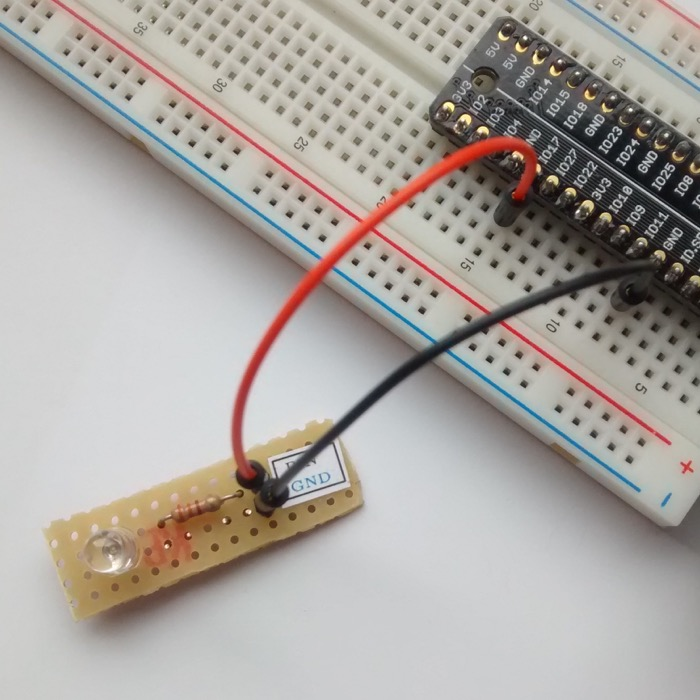
\includegraphics[width=0.8\textwidth]{img/rpCollection/diode.jpg}
	\caption{Diode (LED)
	
	Klasse: \texttt{RPDiode}}
\end{figure}

\column{.45\textwidth}
\begin{figure}[t]
	\centering
	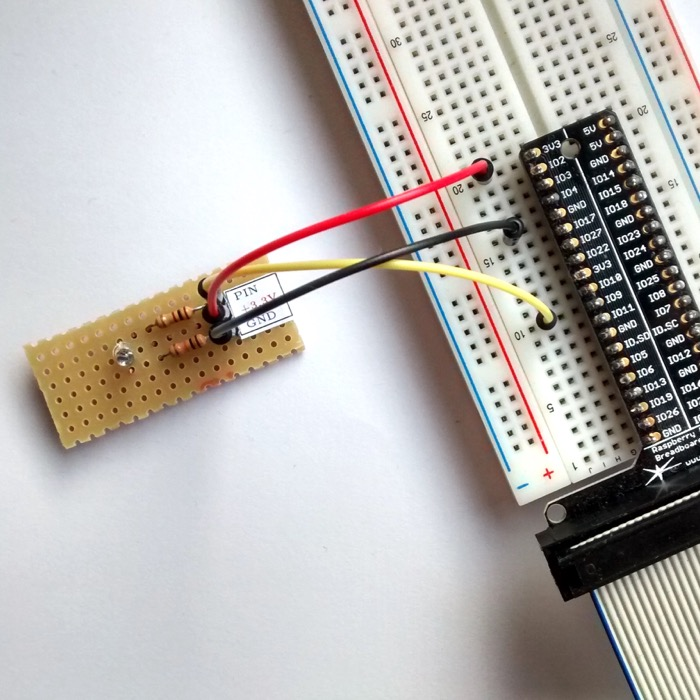
\includegraphics[width=0.8\textwidth]{img/rpCollection/phototransistor.jpg}
	\caption{Phototransistor
	
	Klasse: \texttt{RPPhototransistor}}
\end{figure}
\end{columns}
\end{frame}

% ----------------------------------------------------------

\begin{frame}
\frametitle{Die Bauteile}

\begin{columns}[t]
\column{.45\textwidth}
\begin{figure}[t]
	\centering
	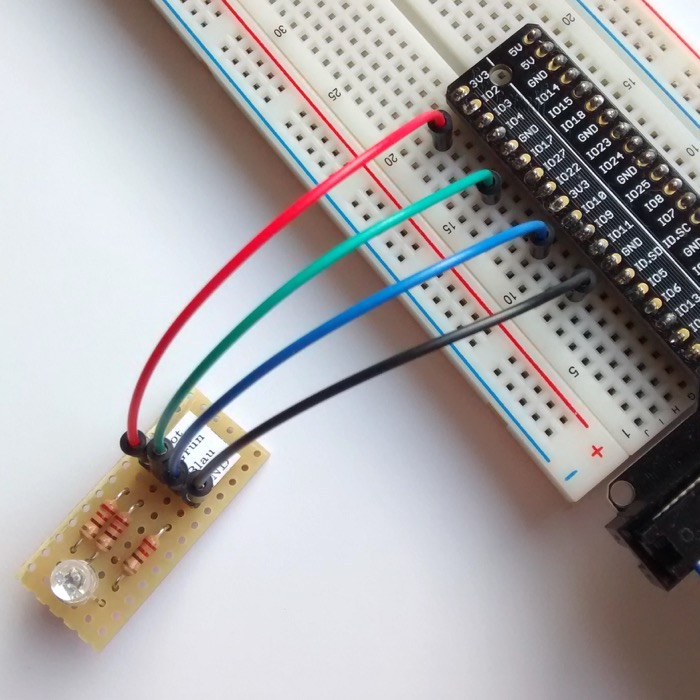
\includegraphics[width=0.8\textwidth]{img/rpCollection/rgbled.jpg}
	\caption{RGB-LED
	
	Klasse: \texttt{RPRGB}}
\end{figure}

\column{.45\textwidth}
\begin{figure}[t]
	\centering
	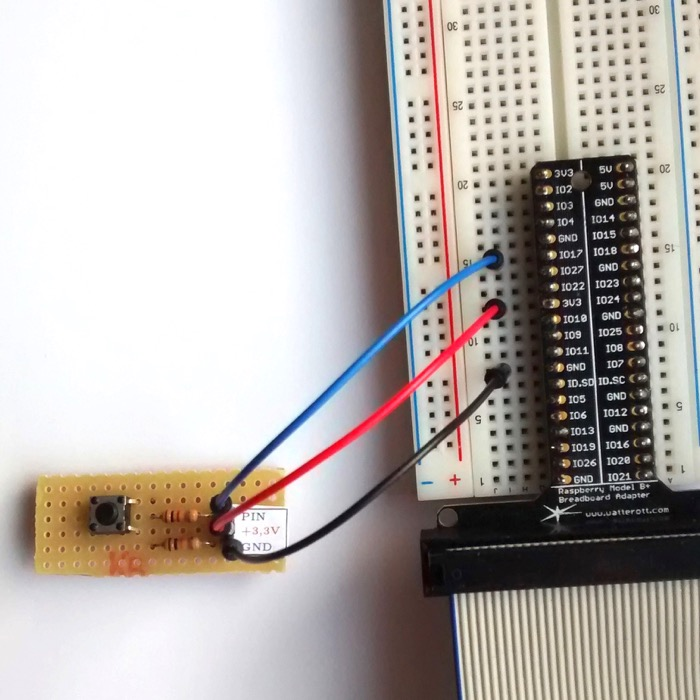
\includegraphics[width=0.8\textwidth]{img/rpCollection/taster.jpg}
	\caption{Taster
	
	Klasse: \texttt{RPTaster}}
\end{figure}
\end{columns}
\end{frame}

% ----------------------------------------------------------

\begin{frame}
\frametitle{Die Bauteile}

\begin{columns}[t]
\column{.45\textwidth}
\begin{figure}[t]
	\centering
	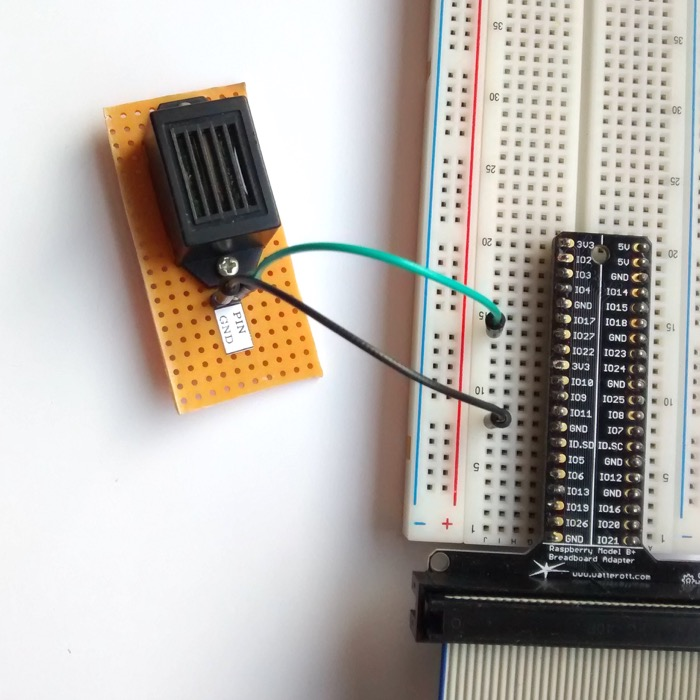
\includegraphics[width=0.8\textwidth]{img/rpCollection/summer.jpg}
	\caption{Summer
	
	Klasse: \texttt{RPSummer}}
\end{figure}

\column{.45\textwidth}
\begin{figure}[t]
	\centering
	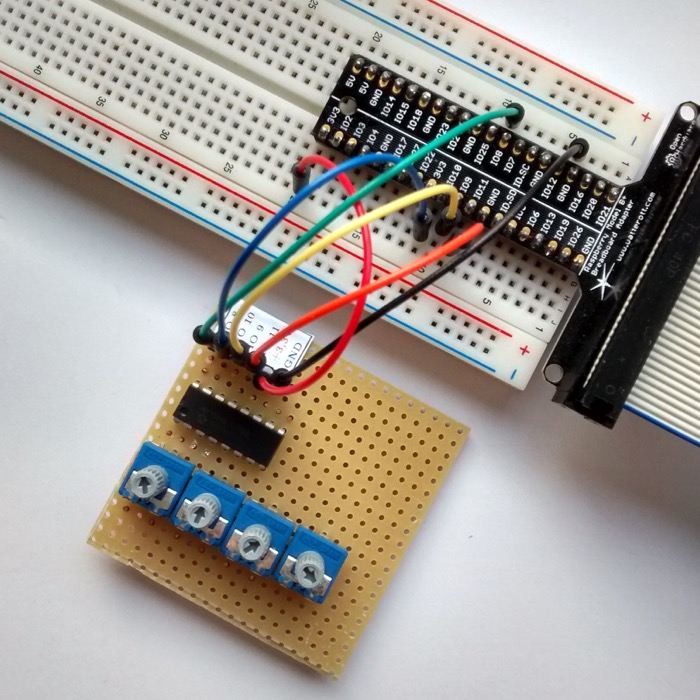
\includegraphics[width=0.8\textwidth]{img/rpCollection/adwandler.jpg}
	\caption{AD-Wandler
	
	Klasse: \texttt{RPADWandler}}
\end{figure}
\end{columns}
\end{frame}

% ----------------------------------------------------------

%\begin{frame}
%\frametitle{Die Bauteile}
%
%\begin{columns}[t]
%\column{.45\textwidth}
%\begin{figure}[t]
%	\centering
%	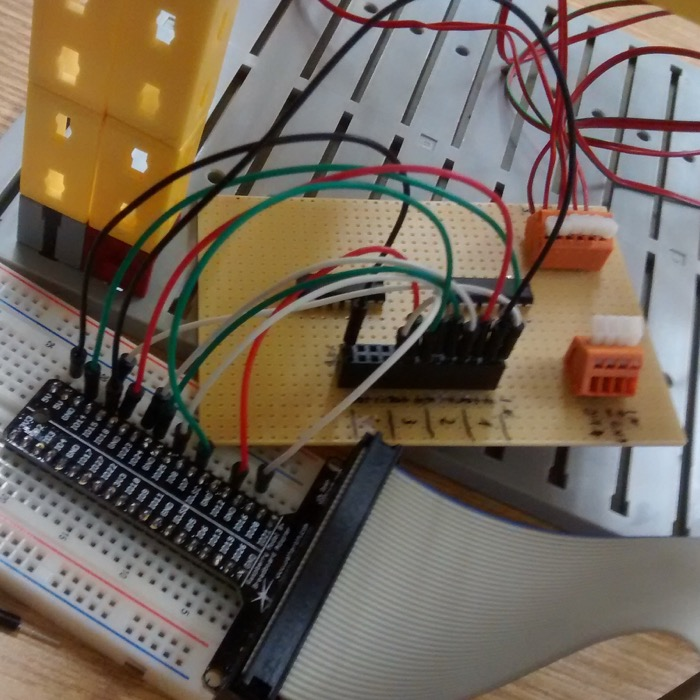
\includegraphics[width=0.8\textwidth]{img/rpCollection/motor.jpg}
%	\caption{Motor
%	
%	Klasse: \texttt{RPMotor}}
%\end{figure}
%
%\end{columns}
%\end{frame}

% ----------------------------------------------------------

\begin{frame}{Der Raspberry Pi}
	\begin{itemize}
		\item Anschluss an bestehende USB-Tastatur, -Maus, HDMI-Monitor, WLAN
		\item Strom über USB-Netzteil
		\item Diverse andere Anschlüsse -- u.\,a. 40-Pin \textbf{GPIO} zum Anschluss der Bauteile
		\item Kosten: ca. \EUR{36} (exkl. Steckbrett, Kabel, Kosten für Bauteile)
	\end{itemize}

	\begin{figure}[ht]
		\centering
		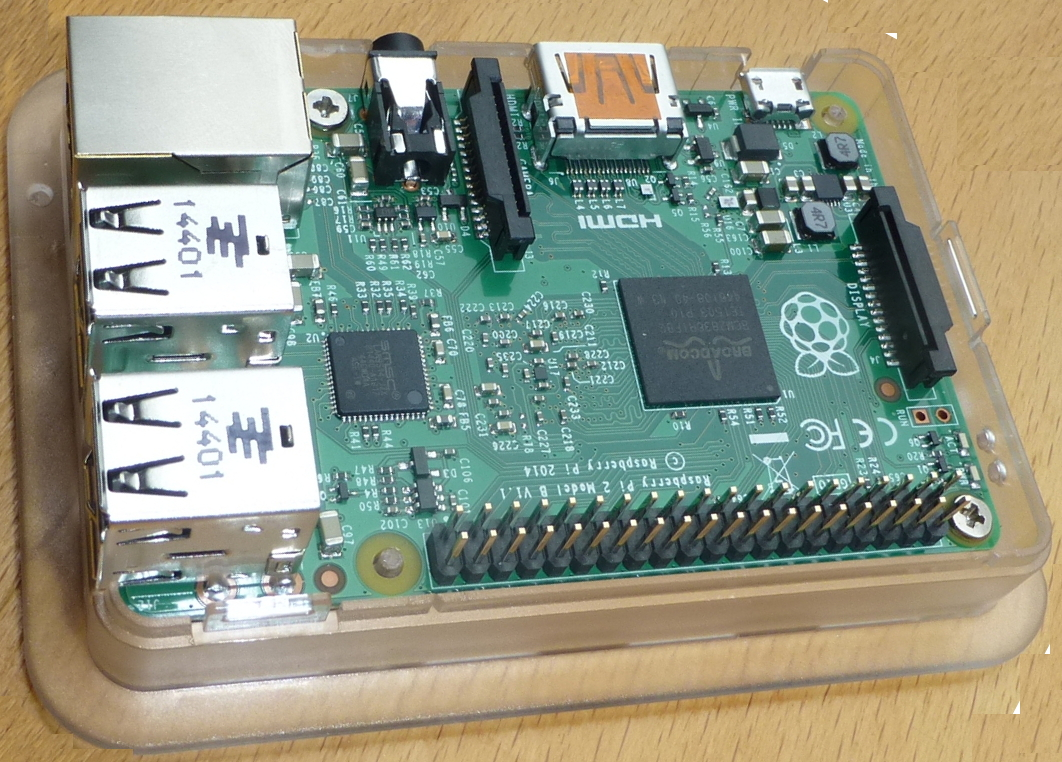
\includegraphics[width=0.5\textwidth]{img/raspi-2b}
		\caption{Raspberry Pi Model 3B.}
	\end{figure}
\end{frame}

% ----------------------------------------------------------

\begin{frame}{Der GPIO}
	\begin{minipage}[t][2cm]{\textwidth}
		\begin{itemize}
			\item 40-Pin GPIO am Raspberry Pi
			\item Ermöglicht den Anschluss von Bauteilen / Sensoren / Steuerungen an frei programmierbare Pinne
			\item<2-> Kabelanschlüsse über ein Steckbrett
		\end{itemize}
	\end{minipage}

	\begin{minipage}[t][6.1 cm]{\textwidth}
		\only<1>{
			\begin{figure}[ht]
				\centering
				\scalebox{.9}{%
					\input{img/gpio_belegung_2b.cir}
				}
				\caption{Der GPIO}
			\end{figure}
		}
		\only<2>{
			\begin{columns}[t]
				\column{.45\textwidth}
					\begin{figure}[t]
						\centering
						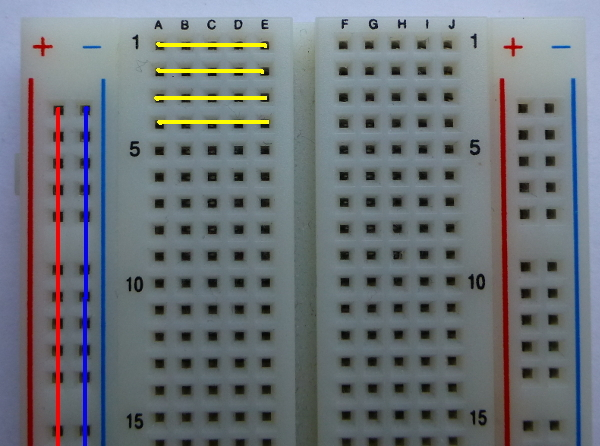
\includegraphics[scale=0.5]{img/steckbrett_leiter.jpg}
						\caption{Interne Belegung}
					\end{figure}
				\column{.45\textwidth}
					\begin{figure}[t]
						\centering
						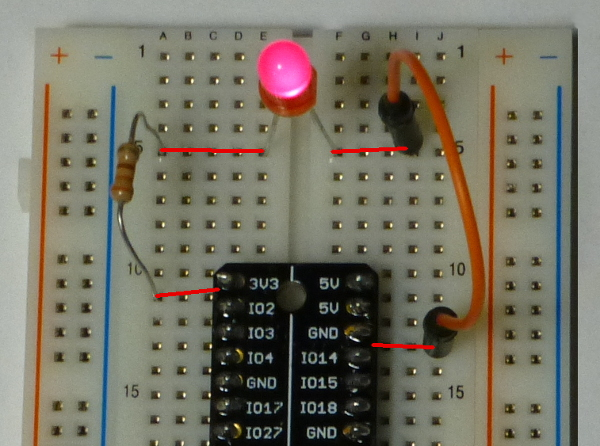
\includegraphics[scale=0.5]{img/steckbrett_led.jpg}
						\caption{Angeschlossene LED}
					\end{figure}
			\end{columns}
		}
		\only<3>{
			\begin{columns}[t]
				\column{.45\textwidth}
					\begin{figure}[t]
						\centering
						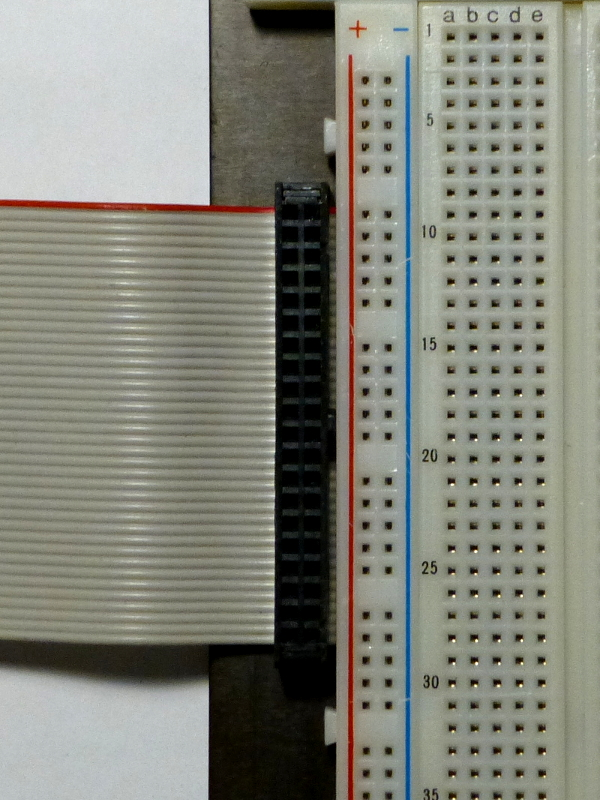
\includegraphics[scale=0.4]{img/steckbrett_kabel.jpg}
						\caption{Festplattenkabel}
					\end{figure}
				\column{.45\textwidth}
					\begin{figure}[t]
						\centering
						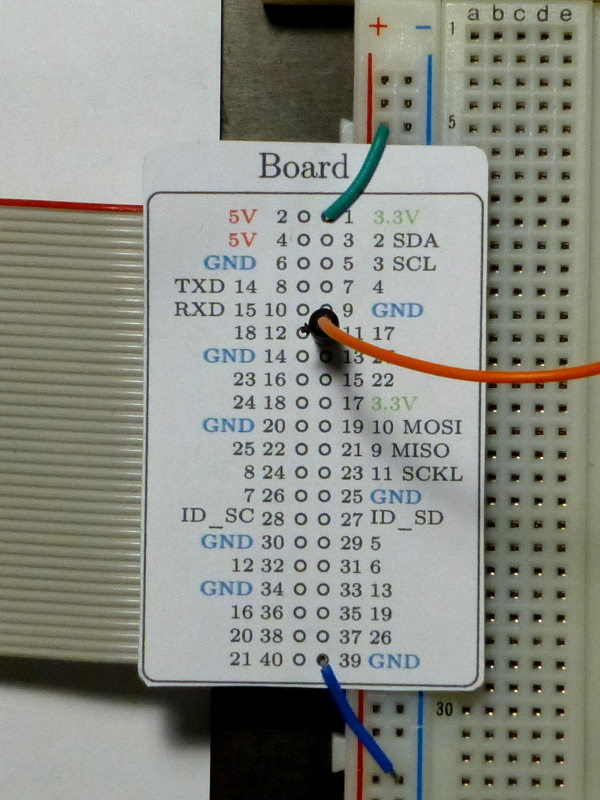
\includegraphics[scale=0.4]{img/steckbrett_zettel.jpg}
						\caption{Mit Belegung}
					\end{figure}
			\end{columns}
		}
	\end{minipage}
\end{frame}

% ----------------------------------------------------------

\subsection{Funktionsweise}

% ----------------------------------------------------------

\begin{frame}
\frametitle{Bauteile steuern: Groovy?}
\begin{itemize}
\item Setzt auf \textbf{Java} (nahtlose Java-Integration)
\item Eigene Programmiersprache 
\item Ungetypt (und weniger streng als Java)
\item \textbf{Groovy = Java ohne Ballast} (Typen, Sichtbarkeitsbereiche, \lstinline|main|-Methode etc.)
\end{itemize}

\vspace{-1.5em}
\begin{figure}[t]
	\centering
	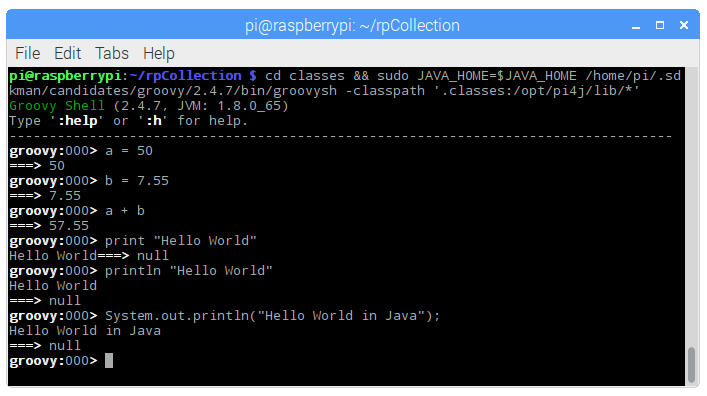
\includegraphics[width=0.5\textwidth]{img/groovysh_einfache_eingaben.png}
	\caption{Einfache Ein- und Ausgaben in der Shell (\texttt{groovysh}).}
\end{figure}
\end{frame}

% ----------------------------------------------------------

\begin{frame}
\frametitle{Groovy-Shell / \texttt{groovysh}}
\vspace{-1em}
\begin{figure}[t]
	\centering
	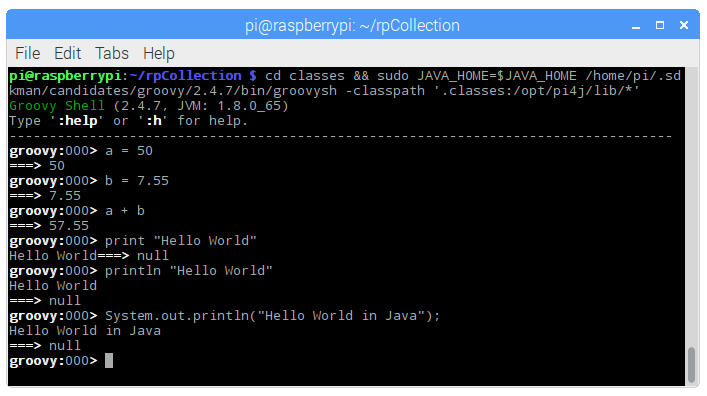
\includegraphics[width=1.0\textwidth]{img/groovysh_einfache_eingaben.png}
	\caption{Einfache Ein- und Ausgaben in der Shell ({groovysh}).}
\end{figure}
\end{frame}

% ----------------------------------------------------------

\begin{frame}
\frametitle{Groovy!}
\begin{itemize}
\item komfortabel nutzbar: Die Groovy-Konsole (\texttt{groovyConsole}) 
\item Für die Schule wurden Start-Skripte geschrieben, weil u.\,a. Pakete eingebunden werden müssen, um mit dem GPIO des Raspberry Pi zu kommunizieren (Pi4J, WiringPi)
\end{itemize}

\begin{figure}[t]
	\centering
	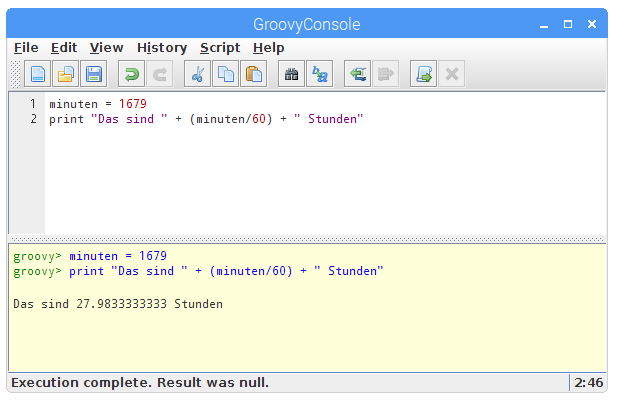
\includegraphics[width=0.5\textwidth]{img/groovyConsole_einfache_eingaben.png}
	\caption{Einfache Ein- und Ausgaben mit GUI (\texttt{groovyConsole}).}
\end{figure}
\end{frame}

% ----------------------------------------------------------

\begin{frame}
\frametitle{\texttt{groovyConsole}}
\vspace{-1em}
\begin{figure}[t]
	\centering
	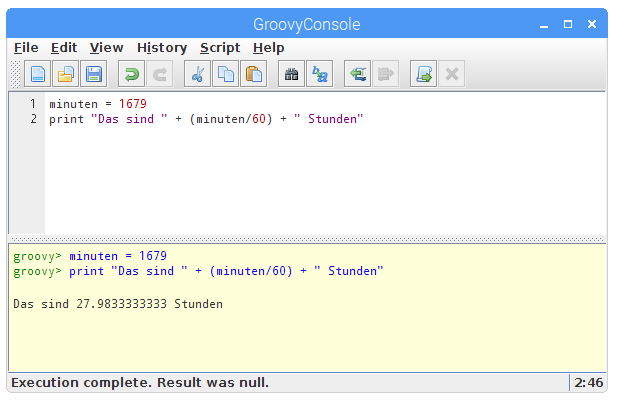
\includegraphics[width=1.0\textwidth]{img/groovyConsole_einfache_eingaben.png}
	\caption{Einfache Ein- und Ausgaben in der Konsole (groovyConsole).}
\end{figure}
\end{frame}

% ----------------------------------------------------------

\begin{frame}[containsverbatim]
\frametitle{Ein Beispiel!}
\begin{block}{Klassischer Java-Code}
\lstset{language=Java}
\begin{lstlisting}[numbers=left, stepnumber=1, numberstyle =\tiny\color{black!30}]
public class manipulator{ 
    public static void main(String[] args){
        RPDiode meinLicht;
        meinLicht = new RPDiode();
        meinLicht.setPin(17);
        meinLicht.blinke();
    }
}
\end{lstlisting}
\end{block}

\vspace{-2mm}
\begin{block}{Groovy (Eingaben auch ohne Semikola möglich)}
\lstset{language=Java}
\begin{lstlisting}[numbers=left, stepnumber=1, numberstyle =\tiny\color{black!30}]
meinLicht = new RPDiode();
meinLicht.setPin(17);
meinLicht.blinke();
\end{lstlisting}
\end{block}
\end{frame}

% ----------------------------------------------------------

\begin{frame}<1>[label=demo,fragile]{Erste Demo!}
	\begin{columns}[t]
		\column{.4\textwidth}
			\textbf{Aufgaben}
			\begin{itemize}
				\item Raspberry Pi kennenlernen
				\item Anschluss von Steckbrett
				\item Anschluss einer Diode
				\item Starten des Pis
				\item Starten der GroovyConsole über das Terminal
				\item Lampe blinken lassen\newline (s. rechts)
			\end{itemize}

		\column{.6\textwidth}
			\textbf{Hilfen}
			\begin{block}{Starten\ldots}
				\lstset{language=Bash}
				\begin{lstlisting}[numbers=left, stepnumber=1, numberstyle =\tiny\color{black!30}, gobble=10]
					cd ~/rpCollection
					./start.sh
				\end{lstlisting}
			\end{block}

			\begin{block}{Blinke blinke (Achtung Pin!)}
				\lstset{language=Java}
				\begin{lstlisting}[numbers=left, stepnumber=1, numberstyle =\tiny\color{black!30}, gobble=10]
					//Mehrfachausfuehrung:
					Helfer.herunterfahren()

					meinLicht = new RPDiode()
					meinLicht.setPin(11)
					meinLicht.blinke()
				\end{lstlisting}
			\end{block}
	\end{columns}
\end{frame}

% ----------------------------------------------------------

\begin{frame}[plain]
	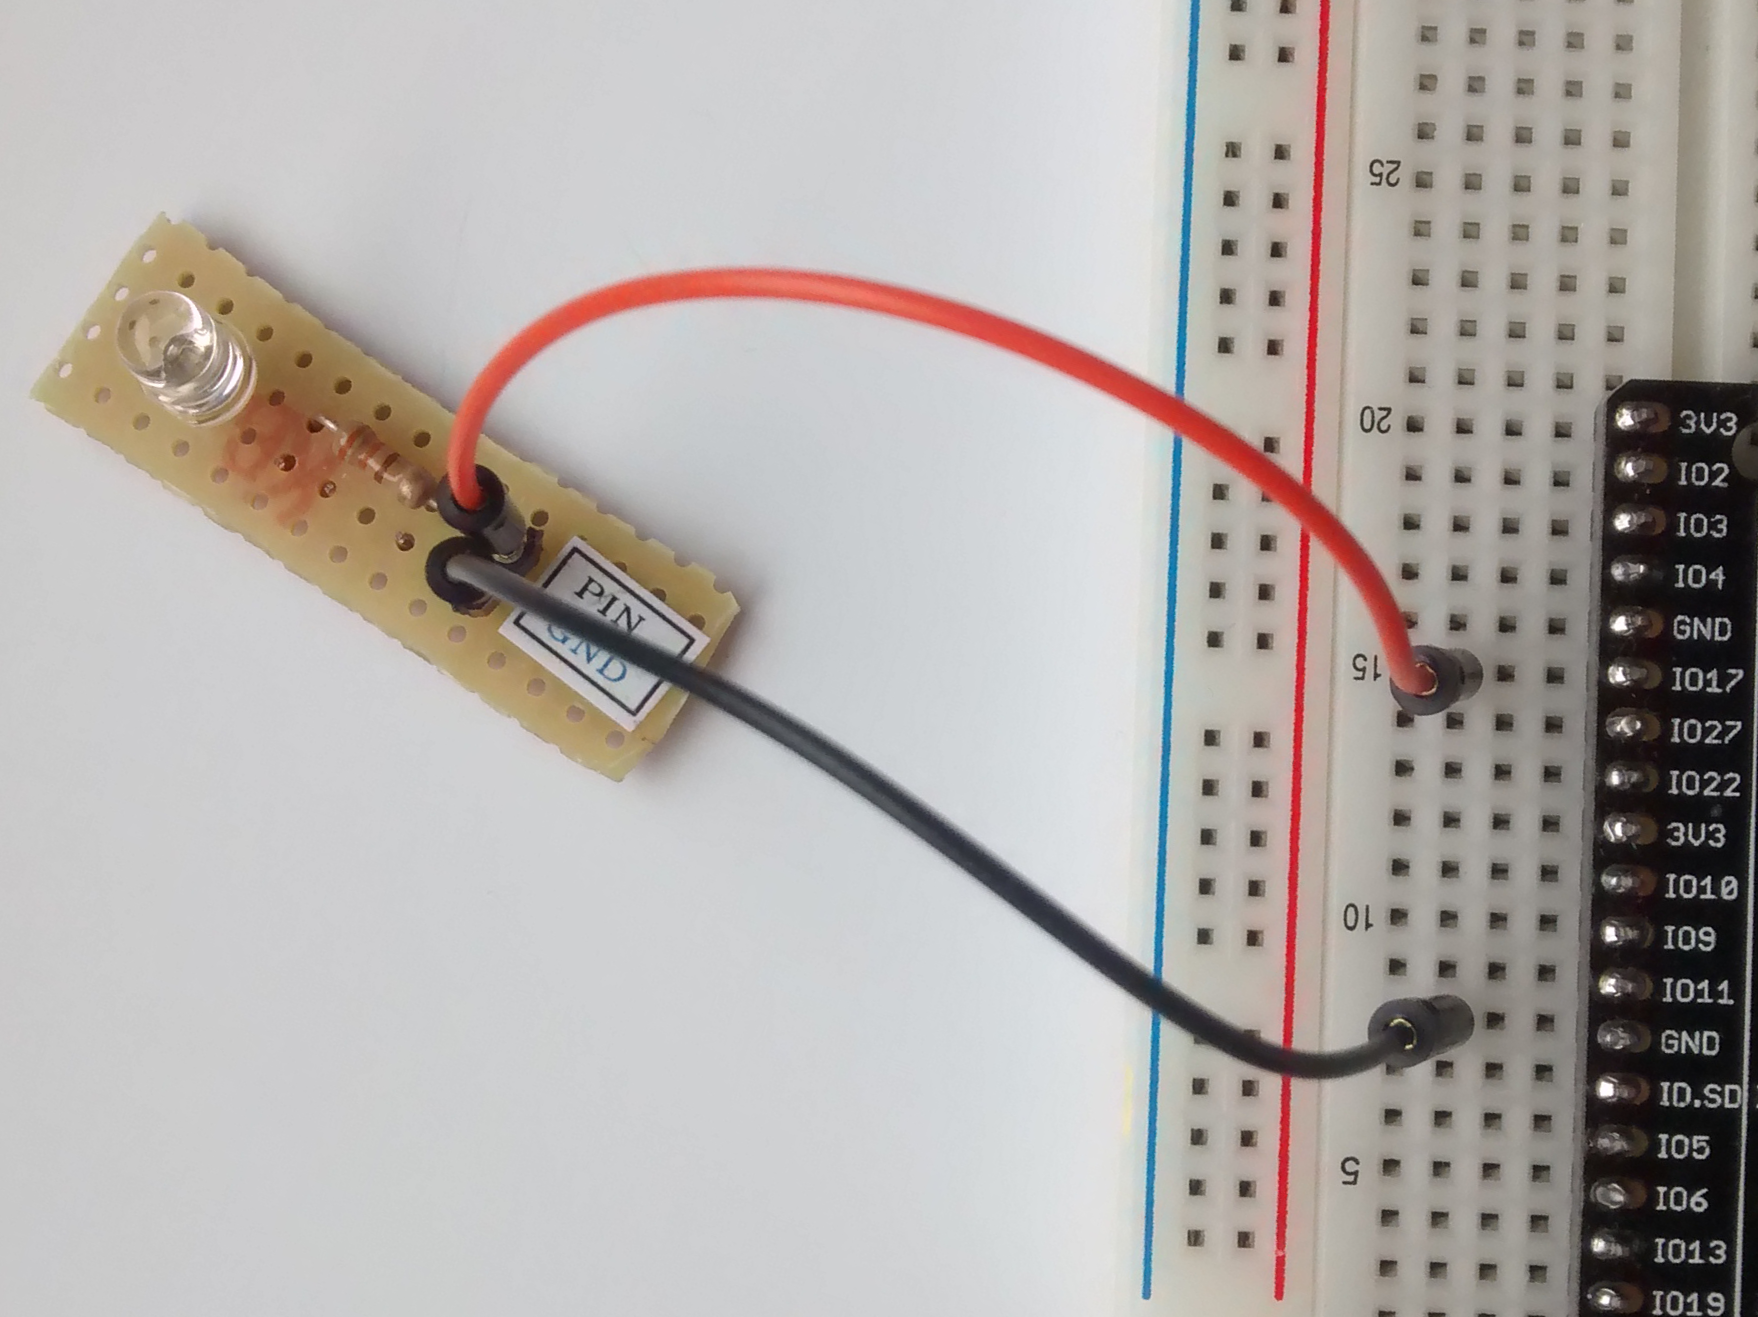
\includegraphics[width=\textwidth]{img/anschluss_diode_an_pin_17}
\end{frame}

% ----------------------------------------------------------

\againframe<2>{demo}

% ----------------------------------------------------------

\begin{frame}
\frametitle{Eingaben in der Konsole}
\vspace{-1.5em}
\begin{figure}[t]
	\centering
	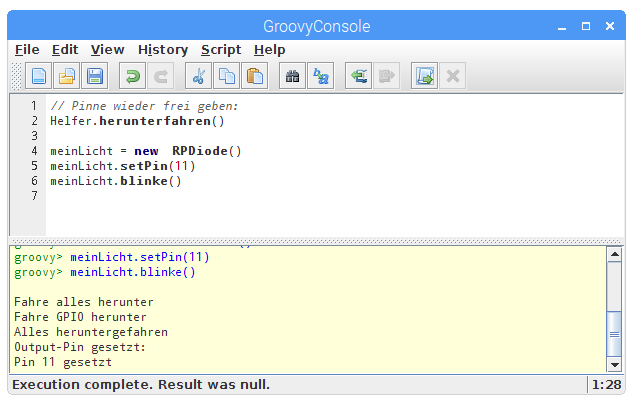
\includegraphics[width=1.0\textwidth]{img/groovyConsole_rpCollection_blinkende_diode.png}
	\caption{Umsetzung in der \texttt{groovyConsole}.}
\end{figure}
\end{frame}

% ----------------------------------------------------------

\begin{frame}
\frametitle{Groovy-Shell}
\vspace{-1.5em}
\begin{figure}[t]
	\centering
	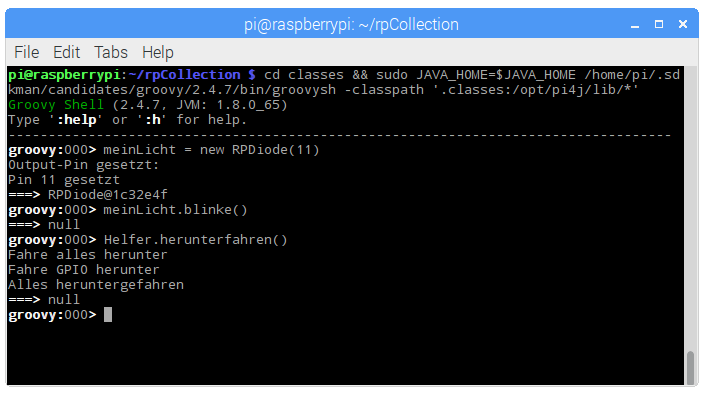
\includegraphics[width=1.0\textwidth]{img/groovysh_rpCollection_blinkende_diode.png}
	\caption{Umsetzung in der Groovy-Shell / in \texttt{groovysh}.}
\end{figure}
\end{frame}

% ----------------------------------------------------------

\begin{frame}
\frametitle{\texttt{groovyShell} (vergrößert)}
\vspace{-0.2em}
\begin{figure}[t]
	\centering
	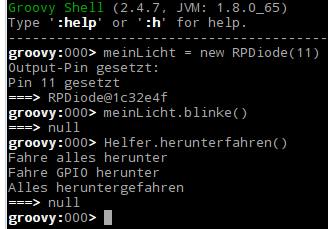
\includegraphics[width=0.95\textwidth]{img/groovysh_rpCollection_blinkende_diode_text_only.png}
	\caption{Umsetzung in der Groovy-Shell / in \texttt{groovysh}.}
\end{figure}
\end{frame}

% ----------------------------------------------------------

\section{Problemstellungen in der Schule}

% ----------------------------------------------------------

\begin{frame}{Objektorientierte Modellierung -- Vorüberlegungen}
	\begin{itemize}
		\item SuS modellieren eine Problemstellung anhand einer Geschichte
		\item Die Modellierung wird mit dem Objektspiel überprüft
		\item Die SuS lernen erst einmal keine Klassen kennen, sondern arbeiten rein auf Objekt-Ebene (\enquote{Objects first}-Ansatz)
		\item Klassen werden zu einem späteren Zeitpunkt eingeführt
		\item Namensgebung an die Entscheidungen der SuS angepasst:
		\begin{itemize}
			\item z.\,B. \texttt{Scheinwerfer} statt \texttt{Diode}; dementsprechend wurden Wrapper-Klassen geschrieben (Klasse \texttt{Scheinwerfer} für \texttt{RPDiode})
			\item Heute wird eine Modellierung \enquote{vorgegeben}
		\end{itemize}
	\end{itemize}
\end{frame}

% ----------------------------------------------------------

\subsection{Unterrichtsvorhaben 1}

% ----------------------------------------------------------

\begin{frame}
\frametitle{In der Schule: Theateraufführung}
\begin{itemize}
\item Steuerung der Lichtanlage einer Theatervorstellung
\item Die SuS
\begin{itemize}
\item Modellieren die Problemstellung: Objekte erkennen, Methoden vergeben, Entwürfe validieren
\item Erstellen Objekte in Groovy
\item Treten in Interaktion mit den Objekten (bzw. Bauteilen)
\item Steuern die Lichtanlage selbstständig, können Programmierung selbstständig überprüfen 
\end{itemize}
\item Problemstellung / ABs schon vorbereitet
\end{itemize}
\end{frame}

% ----------------------------------------------------------

\section{Ausprobieren}

% ----------------------------------------------------------

\begin{frame}<1>[label=demo2]{Zweite Demo}
	\begin{block}{Kleine Problemstellung zum Kennenlernen}
		Martin schaltet zunächst den grünen Scheinwerfer an. Nachdem er etwa 20 Sekunden gewartet hat, schaltet er auch den blauen Scheinwerfer an und schaltet den grünen aus. Nach weiteren 10 Sekunden schaltet er das gesamte Licht aus.
		\vspace{0.8em}

		Für die nächste Szene wird die spezielle Hintergrundbeleuchtung aktiviert. Dazu wird ein Helligkeitssenor befragt und mit der Antwort die Hintergrundbeleuchtung geschaltet.
		\vspace{0.8em}

		Dann arbeitet Martin mit dem RGB-Scheinwerfer\footnote{Der RGB-Scheinwerfer kann -- anders als die anderen -- eine beliebige Farbe annehmen. Dazu stellt man den Anteil an Rot, Grün und Blau ein.}: Er stellt eine Farbe von 50\% für grün, 20\% für rot und 25\% für blau ein. [\ldots]
	\end{block}
\end{frame}

% ----------------------------------------------------------

\begin{frame}{Aufgabenstellung}
	\begin{itemize}
		\item[(1)] Entwerfen Sie zu der gegebenen Problembeschreibung mit Hilfe des Verfahrens von \textsc{Abbott} ein objektorientiertes Modell.
		\begin{itemize}
			\item Heraussuchen von Nomen (Objekte), Verben (Methoden) und Adjektiven (Attribute)
		\end{itemize}

		\item[(2)] Notieren Sie die Objekte als Objektkarten.

		\item[(3)] Setzten Sie die Geschichte in Groovy mit den Hardware-Bausteinen um!
		\begin{itemize}
			\item Nutzen Sie die vorbereiteten Klassen / die Modellierung aus der Schule.
			\item Für diese Demo konnten natürlich keine neuen Wrapper-Klassen geschrieben werden.
		\end{itemize}
	\end{itemize}
\end{frame}

% ----------------------------------------------------------

\againframe<2>{demo2}

% ----------------------------------------------------------

\begin{frame}{Objekte}
	\begin{figure}[htb]
		\centering
		\scalebox{0.58}{
			\begin{tikzpicture}[remember picture]
				\begin{object}[text width=5cm]{martin}{0,0}
					\attribute{~}
					\operation{warte(zeit)}
				\end{object}

				% =========

				\begin{object}[text width=5cm]{scheinwerfer}{0,-2}
					\attribute{standort = \diastring{links}}
					\attribute{farbe = \diastring{blau}}
					\attribute{status = true}

					\operation{anschalten()}
					\operation{ausschalten()}
					\operation{blinken()}
					\operation{schalten(Status)}
					\operation{gibFarbe()}
					\operation{gibStandort()}
					\operation{gibStatus()}
					\operation{setzeFarbe(Farbe)}
					\operation{setzeStandort(Standort)}
					\operation{setzeStatus(Status)}
				\end{object}

			% =========
			% =========
			% =========

				\begin{object}[text width=6cm]{hintergrundbeleuchtung}{6,0}
					\attribute{standort = \diastring{Martins Bühne}}
					\attribute{status = true}

					\operation{schalten(Status)}
					\operation{anschalten()}
						%\operation{bedingtesAnschalten()}	nur wenn Helligkeitssensor bekannt ist sinnvoll (nächste Folie)
					\operation{schalten(Status)}
					\operation{ausschalten()}
					\operation{gibStandort()}
					\operation{gibStatus()}
					\operation{setzeStandort(Standort)}
					\operation{setzeStatus(Status)}
				\end{object}

			% =========

				\begin{object}[text width=6cm]{helligkeitssensor}{6,-6}
					\attribute{standort = \diastring{Bühne}}
					\attribute{status = true}

					\operation{befragenIstHell()}
					\operation{gibStandort()}
					\operation{gibStatus()}
					\operation{setzeStandort(Standort)}
					\operation{setzeStatus(Status)}
				\end{object}

			% =========
			% =========
			% =========

				\begin{object}[text width=5cm]{rgbScheinwerfer}{12,0}
					\attribute{standort = \diastring{Bühnenrand}}
					\attribute{status = true}
					\attribute{farberot = 40}
					\attribute{farbegruen = 70}
					\attribute{farbeblau = 17}

					\operation{einschalten(Rot, Gruen, Blau)}
					\operation{mischen(Rot, Gruen, Blau)}
					\operation{schalten(Status)}
					\operation{ausschalten()}
					\operation{gibStandort()}
					\operation{gibStatus()}
					\operation{gibFarbeRot()}
					\operation{gibFarbeGruen()}
					\operation{gibFarbeBlau()}
					\operation{setzeStandort(Standort)}
					\operation{setzeStatus(Status)}
				\end{object}

			% =========

				\begin{class}[text width=5cm]{Helfer}{12,-9}
					\attribute{~}
					\operation{herunterfahren()}
					\operation{warte(Zeit)}
				\end{class}

			\end{tikzpicture}
			}
			\caption{Objekte mit ihren Attributen und Methoden nach Modellierung der SuS (ohne Konstruktoren $\rightarrow$ dort Pin(ne) angeben!). Auch dargestellt:  Klasse \texttt{Helfer}.}
		\label{fig:objektiagramm_komplett}
	\end{figure}
\end{frame}

% ----------------------------------------------------------

\begin{frame}
\frametitle{Alternativ (Hintergrundbel. kennt den Helligkeitssensor)}

\begin{figure}[htb]
\centering
\scalebox{0.7}{
\begin{tikzpicture}[remember picture]
\begin{object}[text width=7cm]{martin}{0,0}
    \attribute{bekannteHintergrundbeleuchtung = \anchormark{verlinkungMartinHG}[0.025]}
    \operation{warte(zeit)}
\end{object}

\begin{object}[text width=7.3cm]{hintergrundbeleuchtung}{4,-2.5}
    \attribute{bekannterHelligkeitssensor = \anchormark{verlinkungHGSensor}[0.025]}
    \operation{setzeHelligkeitssensor(helligkeitssensor)}
    \operation{bedingtesAnschalten()}
    \operation{anschalten()}
    \operation{ausschalten()}
\end{object}

\begin{object}[text width=5cm]{helligkeitssensor}{8,-6.5}
    \attribute{~}
    \operation{befragenIstHell()} 
\end{object}

\draw[->]  (verlinkungMartinHG.east) -- ($(verlinkungMartinHG.east) + (1.5,0)$) -| ($(hintergrundbeleuchtung.north)+(1,0)$);

\draw[->]  (verlinkungHGSensor.east) -- ($(verlinkungHGSensor.east) + (2,0)$) -| ($(helligkeitssensor.north)+(1,0)$);
\end{tikzpicture}
}
\caption{\textbf{Schalten der Hintergrundbel.}: Martin kennt nur die Hintergrundbeleuchtung und diese den Helligkeitssensor. Es werden nur die wichtigsten Attribute und Methoden dargestellt.}
\label{fig:objektiagramm_hintergrundbel_helligkeitssensor_neue_modellierung}
\end{figure}

\end{frame}

% ----------------------------------------------------------

\section{Diskussion}

% ----------------------------------------------------------

\begin{frame}
\frametitle{Meinungsaustausch und Diskussion}
\begin{itemize}
\item Was hat gut gefallen?
\item Was ist verbesserungswürdig?
\item Wie fanden Sie sich zurecht?
\item \ldots
\end{itemize}
\end{frame}

% ----------------------------------------------------------

\section{Erfahrungen aus der Schule}

% ----------------------------------------------------------

\begin{frame}
\frametitle{Was bleibt den SuS im Gedächtnis?}
\begin{itemize}
\item Die SuS bekommen eine Vorstellung von \textbf{Objekten} mit ihren \textbf{Attributen} und \textbf{Methoden}
\item Die SuS erkennen, dass es Methoden mit und ohne \textbf{Rückgaben} gibt
\item Die SuS können erkennen, dass manche Methoden mit \textbf{Parametern} aufgerufen werden müssen
\item Die SuS können alle Modellierungs- und Beziehungsentscheidungen selbst treffen, um die Geschichte umzusetzen
\end{itemize}
\end{frame}

% ----------------------------------------------------------

\subsection{Vor- und Nachteile des vorgestellten Ansatzes}

% ----------------------------------------------------------

\begin{frame}
\frametitle{Vor- und Nachteile}

\begin{columns}[t]
\column{.45\textwidth}
\textbf{Vorteile}
\begin{itemize}
\item Motivation durch Hardware
\item Sehen von Attributwerten
\item Sehen / Hören von Ergebnissen von Methodenaufrufen
\item Selbstüberprüfung / Hilfe zur Selbsthilfe
\item Lebensnahe Beispiele
\item kostengünstige Anschaffung
\end{itemize}

\column{.45\textwidth}
\textbf{Nachteile}
\begin{itemize}
\item SuS sind sehr fixiert auf die Bauteile
\item Ablenkung durch andere Möglichkeiten der Bauteile
\item Einrichtung von Java auf den Pis muss stimmen (Abhilfe: Raspbian-Image vorbereiten und Hilfedatei nutzen)
\end{itemize}
\end{columns}
\end{frame}

% ----------------------------------------------------------

\subsection{Vorerfahrungen mit Informatik und Meinungen der SuS}

% ----------------------------------------------------------

\begin{frame}
\frametitle{Notwendige Vorerfahrungen?}
\begin{itemize}
\item \textbf{Keine!} 
\item Die SuS lernen langsam die OOM kennen
\item Das Objektspiel hilft, die Modellierung zu \textbf{überprüfen} und \textbf{Beziehungen} zu erkennen bzw. die Geschichte durchzuspielen
\item \textbf{Sequenzdiagramme} und \textbf{Objektdiagramme} werden genutzt, um Informationsfluss bzw. die Modellierung darzustellen
\end{itemize}
\end{frame}

% ----------------------------------------------------------

\begin{frame}
\frametitle{Schülermeinungen}
\begin{itemize}
\item \enquote{[\dots] und außerdem konnte man dann eben auch gucken, sich selbst überprüfen, also ob man es richtig gemacht hat, indem man das dann halt ablaufen lassen hat, und das musste nicht vom Lehrer überprüft werden} (Schüler F)

\item \enquote{Ich glaub schon, dass es mehr Vorteile gibt, weil man halt dadurch selbst auch Sachen ausprobieren kann. Und da viele Leute die Sachen halt besser verstehen, wenn man sie selbst in der Praxis umsetzt, als wenn man sie nur in der Theorie durchnimmt. Und ich persönlich fand das Objektspiel mit den Karten immer sehr verwirrend und hab das nie so ganz verstanden. Aber wenn man das dann halt in diese Groovy Konsole eingegeben hat, wurde es für mich halt immer deutlicher und ich habe es halt besser verstanden. Und da glaub ich halt schon, dass diese (.) Praxisarbeit zum Verständnis beiträgt} (Schüler C)
\end{itemize}
\end{frame}

% ----------------------------------------------------------

\section{Wie geht's weiter?}

% ----------------------------------------------------------

\begin{frame}
\frametitle{Wie geht's weiter?}
\begin{itemize}
\item Auch \textbf{Klassen} können in Groovy modelliert werden
\item An die Problemstellungen kann die Einführung von Klassen angeknüpft werden 
\end{itemize}
\end{frame}

% ----------------------------------------------------------

\subsection{Unterrichtsvorhaben 2}

% ----------------------------------------------------------

\begin{frame}{Eine andere Aufgabe: Hafenkransteuerung}
	\begin{columns}[t]
		\column{.45\textwidth}
		\begin{itemize}
			\item Fischer-Technik Hafenkran
			\item Aktivitäten wie beim Theater, diesmal mehr \enquote{Action}
			\begin{itemize}
				\item es bewegt sich mehr!
				\item Drehen des Krans
				\item Arm heben / senken
				\item Seilwindensteuerung
			\end{itemize}
			\item Problemstellung / ABs schon vorbereitet
		\end{itemize}

		\column{.45\textwidth}
		\begin{figure}[t]
			\centering
			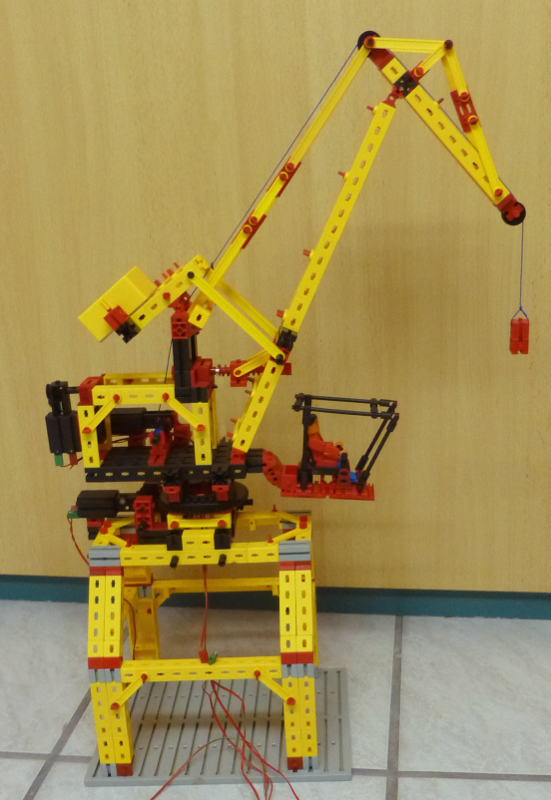
\includegraphics[width=0.7\textwidth]{img/kran}
			\caption{Hafenkran mit drei Motoren.}
		\end{figure}
	\end{columns}
\end{frame}

% ----------------------------------------------------------

\begin{frame}{Weitere Infos}
	\begin{columns}[t]
		\column{.45\textwidth}
		\begin{itemize}
			\item Ätz-Vorlagen für die Platinen
			\item Angedacht / Prinzipiell möglich: Steuerung eines LEGO-Radladers (aber: Anschaffungskosten hoch) durch Motoren-Platinen; Dioden anbauen und schalten (keine Lenkung)
			\item Steuerung anderer Fischertechnik-Bausätze möglich
		\end{itemize}

		\column{.45\textwidth}
		\begin{figure}[t]
			\centering
			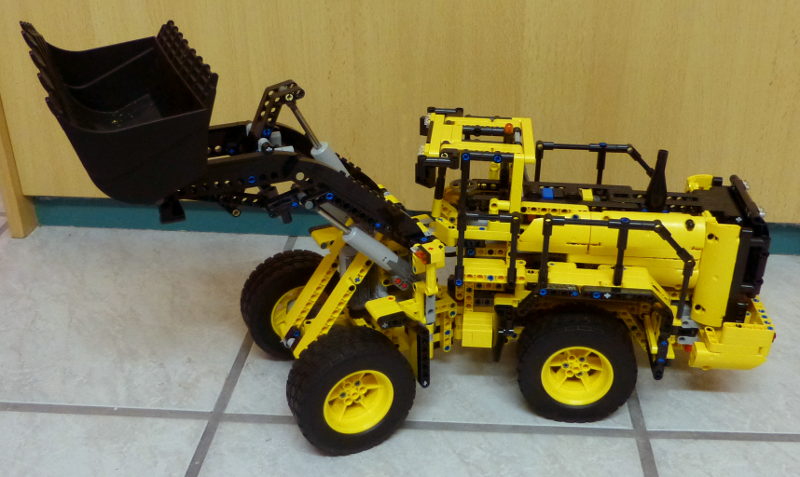
\includegraphics[width=0.9\textwidth]{img/radlader2}
			\caption{LEGO Technic -- Bausatz 42030.}
		\end{figure}
	\end{columns}
\end{frame}

% ----------------------------------------------------------

\begin{frame}
\frametitle{Wie komme ich an das Material?}
\begin{itemize}
\item Alles liegt in einem git-Repository: 

\begin{mdframed}[linecolor=BlueViolet,linewidth=2px]
\begin{center}
\vspace{0.4cm}
\url{https://github.com/hnrstrck/rpCollection}
\vspace{0.4cm}
\end{center}
\end{mdframed}

\item Sämtliche ABs
\item Sämtliche Quelltexte
\item Etiketten für den Nachbau
\item Erklärungen zur Steuerung und zum Nachbau / Anschluss der Bauteile folgen durch die Veröffentlichung der Masterarbeit
\item Bilder der Bauteile
\item Vorlagen für die Platinen
\item Diese Präsentation (\texttt{tex}-Datei)
\end{itemize}
\end{frame}

% ----------------------------------------------------------

\begin{frame}

\vspace{0.5cm}
{\Huge{\centerline{Vielen Dank!}}}

\begin{mdframed}[linecolor=Green,linewidth=1px]
\begin{center}
\vspace{0.2cm}
{\small Diese Präsentation (und ihre Quelldatei/en) und alle im Repository aufgeführten Dateien stehen unter einer \textbf{Namensnennung -- Nicht-kommerziell -- Weitergabe unter gleichen Bedingungen 4.0 International-Lizenz} (sofern nicht anders in der jeweiligen Datei angegeben). Die Bedingungen der Lizenz können unter folgendem Link eingesehen werden:

{\footnotesize \url{http://creativecommons.org/licenses/by-nc-sa/4.0/deed.de}}}

\begin{figure}[b]
	\centering
	\includegraphics[width=0.3\textwidth]{img/img_by-nc-sa-eps-converted-to.pdf}
\end{figure}

\vspace{0.1cm}

\end{center}
\end{mdframed}

\end{frame}

% ----------------------------------------------------------

\begin{frame}
\frametitle{Quellen}
\footnotesize{
\begin{thebibliography}{99}

\bibitem[GitHub Heiner Stroick]{github_heinerstroick} Heiner Stroick: \emph{Java-Objekte zum anfassen (Hardware-Bausteine am Raspberry Pi)}, \url{https://github.com/hnrstrck/rpCollection}, aufgerufen am 01.04.2017.

\bibitem[DDI Wuppertal Übersichtsseite / Materialsammlung]{ddi_wuppertal_uebersicht} Didaktik der Informatik an der Bergischen Universität Wuppertal, \emph{Aktuelles}, \url{http://ddi.uni-wuppertal.de/}, aufgerufen am 27.09.2016.

\bibitem[GI Curriculum 2016]{VorschlagschulinternesCurriculumGI} Gesellschaft für Informatik (Dorothee \textsc{Müller} / Johannes \textsc{Pieper} \etal) (2016): \emph{Informatik: Schulinterner Lehrplan zum Kernlehrplan für die gymnasiale Oberstufe an der Mustergesamtschule in Musterstadt}, \url{http://ddi.uni-wuppertal.de/material/materialsammlung/klp.html}, aufgerufen am 25.07.2016. Direktlink: \url{http://ddi.uni-wuppertal.de/material/materialsammlung/oberstufe/KERNLEHRPLAN/SILP_GOSt_Informatik_Muster.pdf}, aufgerufen am 06.11.2016.

\bibitem[weitere]{weitere} Weitere Quellen für theoretische Grundlagen / praktische Umsetzung: s. Masterarbeit von Heiner Stroick (\enquote{Einstieg in die Objektorientierung mit Unterstützung des Raspberry Pi}, TU Dortmund, Wintersemester 2016 / 2017). Veröffentlichung folgt im entsprechenden Git-Repository (siehe oben).

\end{thebibliography}
}
\end{frame}

% ----------------------------------------------------------

\end{document}